%\newpage

\chapter[METODOLOGIA]{Metodologia}

% Neste capítulo devem ser descritos os procedimentos a serem seguidos na realização da pesquisa. A metodologia depende da natureza do trabalho, do tipo de pesquisa que se pretende desenvolver e, principalmente dos objetivos que se propõem alcançar. De acordo com Gil (2018), na metodologia são apresentadas as seguintes informações: 

% Tipo de pesquisa: esclarecer a natureza (exploratória, descritiva ou explicativa) e o delineamento da pesquisa (experimental, estudo de caso, pesquisa bibliográfica, etc.); 

% População e amostra: apresentar o universo a ser estudado, extensão da amostra e forma de seleção; 

% Coleta de dados: descrever as técnicas a serem utilizadas para coleta de dados (questionários, ensaios laboratoriais, ensaios de campo, técnicas de entrevista ou de observação, etc.); 

% Análise dos dados: descrever os procedimentos a serem adotados para análise quantitativa e/ou qualitativa.

\section{Materiais}

\subsection{Solo}

O solo a ser utilizado foi extraído no município de Pontal do Araguaia, Mato Grosso, em um trecho próximo às margens do contorno viário que liga as rodovias BR-070 e BR-158 à rodovia MT-100. Após a coleta, o material foi encaminhado ao laboratório, onde passou por um preparo prévio consistindo em ser destorroado, descartado a fração de pedregulho e, posteriormente, armazenado em local protegido das intempéries. Trata-se de um material já vastamente estudado e utilizado em pesquisas anteriores desenvolvidas na instituição. Os ensaios o classificam como um material granular do tipo areia siltosa ou argilosa do sistema AASHTO \cite{Barroso2019,Junior2021, Silva2019,Novato2019,Soler2021}. 

\begin{figure}[h]
    \centering
    \label{fig:solo-coletado}
    \caption{Local da coleta do solo.}
    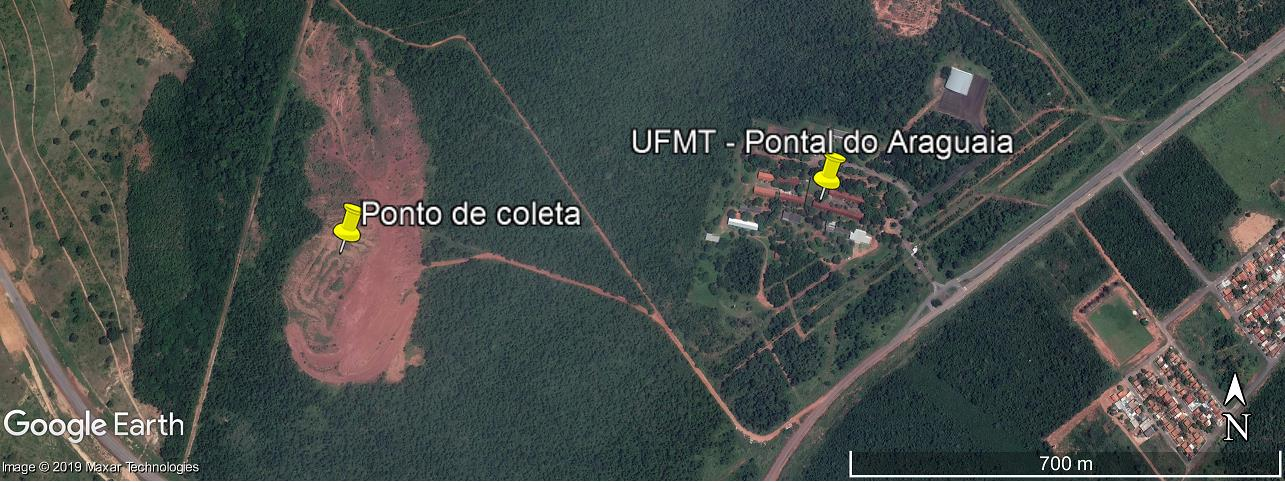
\includegraphics[width=1\textwidth]{assets/images/solo-coletado.jpg}
    \fonte{\citeonline{Barroso2019}}
\end{figure}

%\subsection{Aglomerantes}

\subsection{Cimento}

O aglomerante químico empregado para a estabilização dos adobes será o Cimento Portland Composto com pozolana (CP II-Z 32), material cuja especificação técnica é regida pela \citeonline{nbr11578}. Os teores de cimento avaliados serão de 3\%, 5\% e 7\% em relação à massa de solo seco. A escolha justifica-se pela sua eficácia comprovada em estabilizar solos granulares que empregaram 7\% de cimento \cite{Barroso2023,Soler2024}, além do interesse em investigar a possibilidade de redução do teor de aglomerante sem prejuízo significativo do desempenho mecânico.

\subsection{Hidrofugantes}

A fim de diminuir a extrema vulnerabilidade hídrica do material e preservar a integridade estrutural dos adobes estabilizados sob condições de saturação prolongada, os corpos de prova receberão a aplicação de um tratamento de proteção superficial com aditivos hidrofugantes. Para esse propósito, será empregado um agente hidrofóbico comercial, cuja função é promover o bloqueio externo da rede de capilaridade sem refinar ou alterar a microestrutura interna da matriz de solo-cimento. 

\section{Confecção dos Blocos de Adobe}

\subsection{Preparo da mistura}

O processo produtivo inicia-se com a realização da mistura dos materiais secos e adiciona-se água de forma gradativa. A mistura é homogeneizada até atingir uma consistência plástica, garantindo a coesão necessária para que o bloco não se deforme após o desmolde.

\subsection{Moldagem dos blocos}

A moldagem do adobe é feita manualmente, sobre uma superfície plana isolada por uma lona plástica. Será utilizado moldes vazados com dimensões de 12 cm x 24 cm x 7 cm. Antes de receber a massa, as fôrmas serão obrigatoriamente lubrificadas para evitar a aderência e facilitar a retirada do bloco. A massa plástica é inserida na fôrma em pequenas quantidades, sendo friccionada e comprimida com as mãos de forma a preencher rigorosamente os cantos e evitar a formação de espaços vazios. Após o preenchimento, realiza-se o nivelamento da face superior, retirando-se o excesso de massa com uma régua, procedendo-se com o desmolde imediato através do levantamento vertical da fôrma.

\begin{figure}[h]
    \centering
    \label{fig:moldagem-blocos}
    \caption{Moldagem dos blocos}
    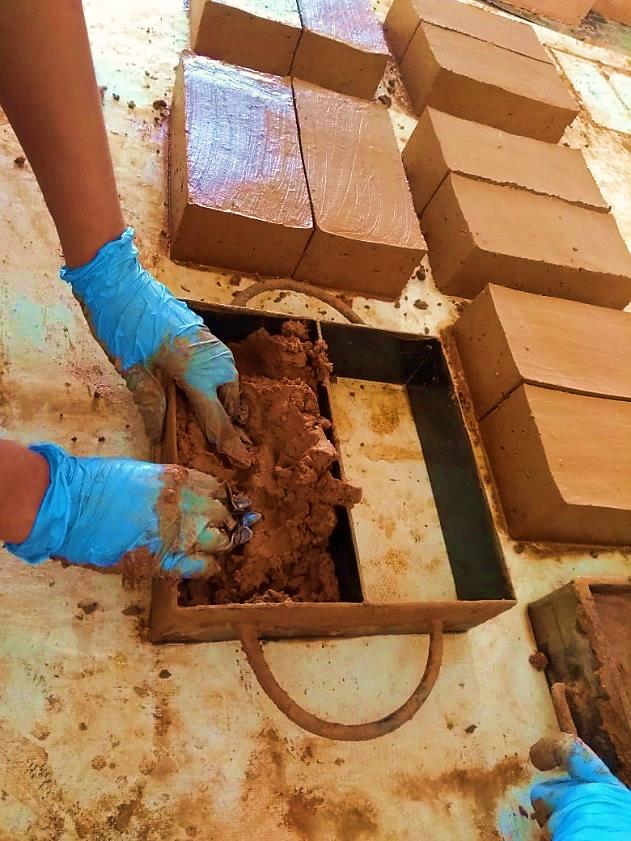
\includegraphics[width=.3\textwidth]{assets/images/moldagem-blocos.jpg}
    \fonte{\citeonline{Barroso2019}}
\end{figure}

\subsection{Processo de cura e secagem}

A cura vai ocorrer à temperatura ambiente e protegido das intempéries. Nos primeiros dias, os tijolos cimentícios devem ser umedecidos ou pulverizados com água diariamente para garantir as reações de hidratação do ligante, o que evita a retração volumétrica severa e a formação de fissuras.

\begin{figure}[h]
    \centering
    \label{fig:cura-blocos}
    \caption{Cura dos adobes}
    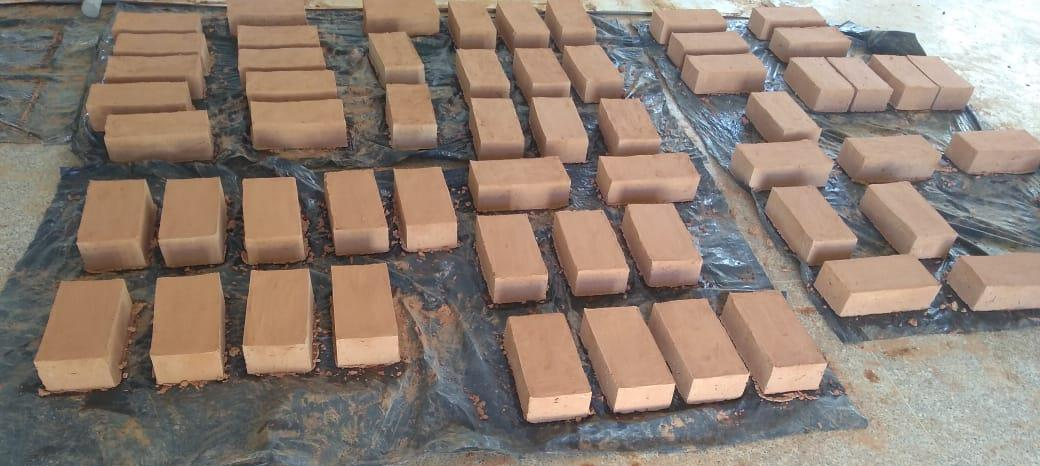
\includegraphics[width=1\textwidth]{assets/images/cura-blocos.jpg}
    \fonte{\citeonline{Silva2019}}
\end{figure}

\section{Ensaios}

\subsection{Resistência a compressão}

A avaliação da capacidade mecânica de carga baseia-se nas recomendações e metodologias da norma \citeonline{nbr8492}. Previamente ao rompimento, a face superior dos blocos deve ser retificada por meio de um capeamento feito com argamassa de cimento e areia (traço de 1:2), respeitando uma espessura máxima de 3 mm e um período de cura de 24 horas, para assegurar o paralelismo da superfície que receberá a força de esmagamento. O corpo de prova é então centralizado na prensa hidráulica posicionado entre duas chapas de aço, o que garante a transferência e a distribuição uniforme da tensão aplicada. O ensaio ocorre sob uma velocidade de carregamento contínua, geralmente adotada como 50 mm/min.

\begin{figure}[htb]
    \centering
    \label{fig:capeamento}
    \caption{Capeamento}
    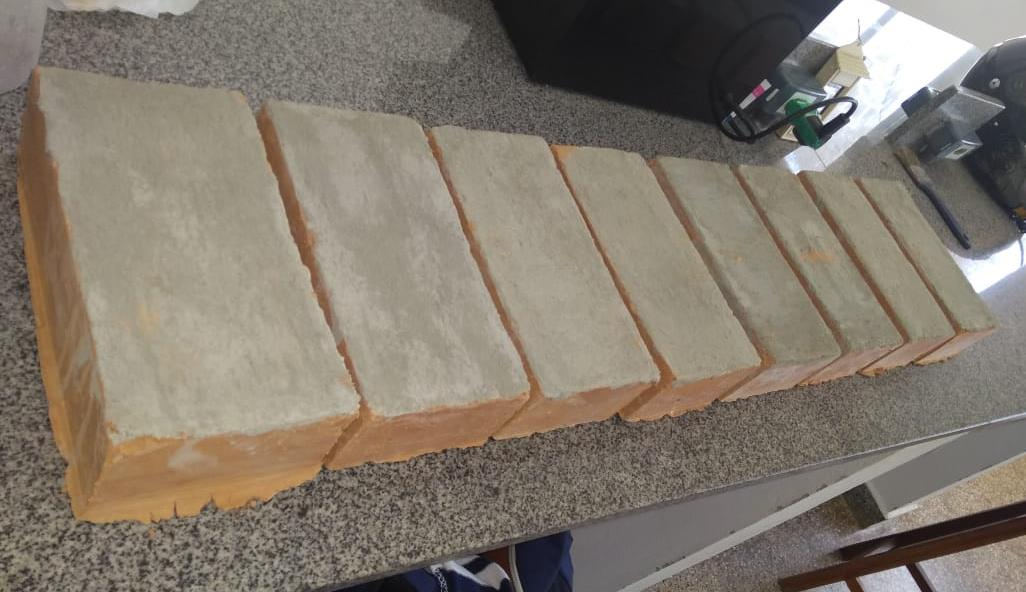
\includegraphics[width=.75\textwidth]{assets/images/capeamento.jpg}
    \fonte{\citeonline{Silva2019}}
\end{figure}

\begin{figure}[htb]
    \centering
    \label{fig:ensaio-compressao}
    \caption{Corpo de prova no ensaio de resistência à compressão}
    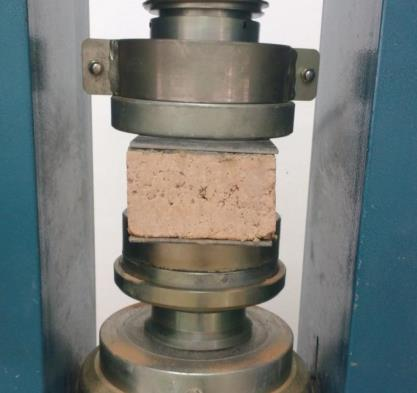
\includegraphics[width=.5\textwidth]{assets/images/ensaio-compressao.jpg}
    \fonte{\citeonline{Schweig2018}}
\end{figure}

Para os grupos controle, imersão e imersão com hidrofugante, serão consideradas as idades de cura de 28, 42 e 56 dias. Além dessas idades, para os adobes de solo-cimento pertencentes aos grupos controle e imersão, também serão realizados ensaios aos 7 e 14 dias de cura, com o objetivo de caracterizar o desenvolvimento da resistência mecânica nas fases iniciais do processo de cura.

Para cada combinação de traço, condição experimental e idade de cura, serão moldados três corpos de prova. Assim, considerando os grupos controle, imersão e imersão com hidrofugante, serão produzidos, ao todo, 117 adobes de solo-cimento.

\subsection{Absorção de água}

Também regido pela \citeonline{nbr8492}, esse ensaio determina a capacidade da matriz porosa em reter água. O procedimento inicia-se com a inserção dos corpos de prova em uma estufa à temperatura de 100 °C por um período de 24 horas, aferindo-se em seguida a sua massa seca ($M_s$). Na sequência, os tijolos são totalmente submersos em água à temperatura ambiente pelo período de 24 horas. Ao término da imersão, os blocos são retirados, secos superficialmente com o auxílio de um tecido úmido para a remoção da água externa e pesados, obtendo-se a massa úmida ($M_u$). O teor de absorção final, expresso em porcentagem:

\begin{equation}
    \text{Teor de absorção (\%)} = \frac{M_u-M_s}{M_s}\times 100
    \label{eq:teor-de-absorção}
\end{equation}

\begin{figure}[htb]
    \centering
    \label{fig:blocos-submersos}
    \caption{Blocos submersos em água}
    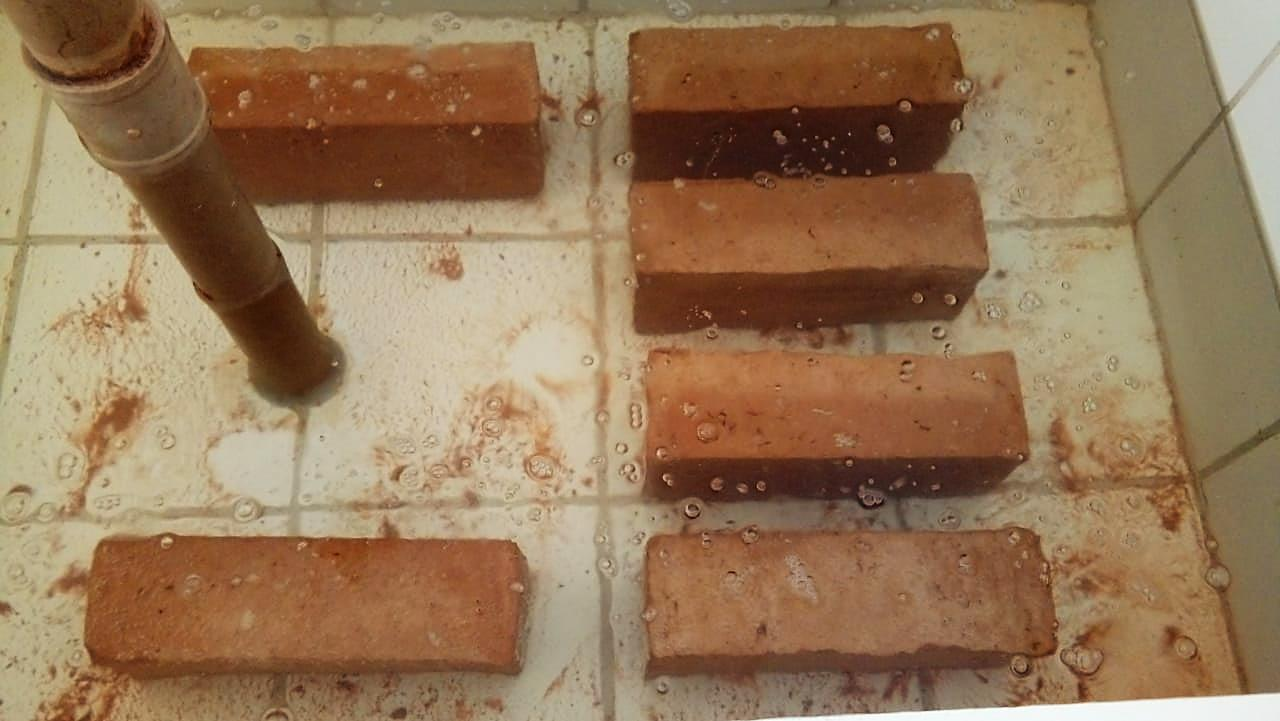
\includegraphics[width=.75\textwidth]{assets/images/blocos-submersos.jpg}
    \fonte{\citeonline{Barroso2019}}
\end{figure}

Serão considerados dois períodos de cura, 7 e 28 dias de cura, para cada traço estudado. Sabendo que, serão confeccionados corpos de prova cilíndricos com 5 cm de diâmetro e 5,3 cm de altura.

\subsection{Retração}

Esse teste afere as variações volumétricas e a propensão à fissuração da mistura durante as fases de secagem, utilizando como base a metodologia proposta por Buson adaptada das recomendações do Centro de Pesquisas e Desenvolvimento (CEPED). A massa de solo, em consistência plástica equivalente à da confecção do adobe, é acondicionada em uma caixa de ensaio vazada, previamente lubrificada, com dimensões internas padronizadas em 3,5 cm de altura, 8,5 cm de largura e 60 cm de comprimento. 

\begin{comment}
\begin{figure}[htb]
    \centering
    \label{fig:ensaio-retração}
    \caption{Representação do processo de acomodação das misturas na caixa de ensaio de retração}
    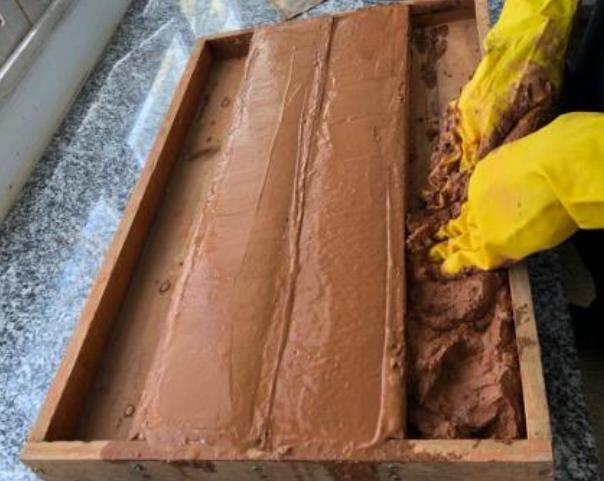
\includegraphics[width=.5\textwidth]{assets/images/ensaio-retracao.jpg}
    \fonte{\citeonline{Soler2024}}
\end{figure}
\end{comment}

Para promover o adensamento e uma distribuição homogênea do material, levanta-se uma das extremidades da caixa até a altura aproximada de 7 cm, soltando-a para cair sob a ação da gravidade, repetindo-se o movimento de impacto por dez vezes consecutivas. A amostra permanece em repouso, protegida do sol, excesso de umidade e intempéries, por 7 dias. Finalizado o tempo de cura, realiza-se a medição do distanciamento gerado nas duas extremidades da caixa para apurar a retração total e afere-se a formação de trincas na superfície. O traço só é validado para utilização em elementos construtivos caso seja isento do surgimento de trincas e registre uma retração linear total que não ultrapasse 2 cm.